\subsection{\label{sec:analysis} Analysis}
In this section, we present several visualizations on DDS. We focus on multilingual NMT, mainly because its data selection distribution is over 8 languages, which is simpler and easier to interpret.  
\begin{center}
  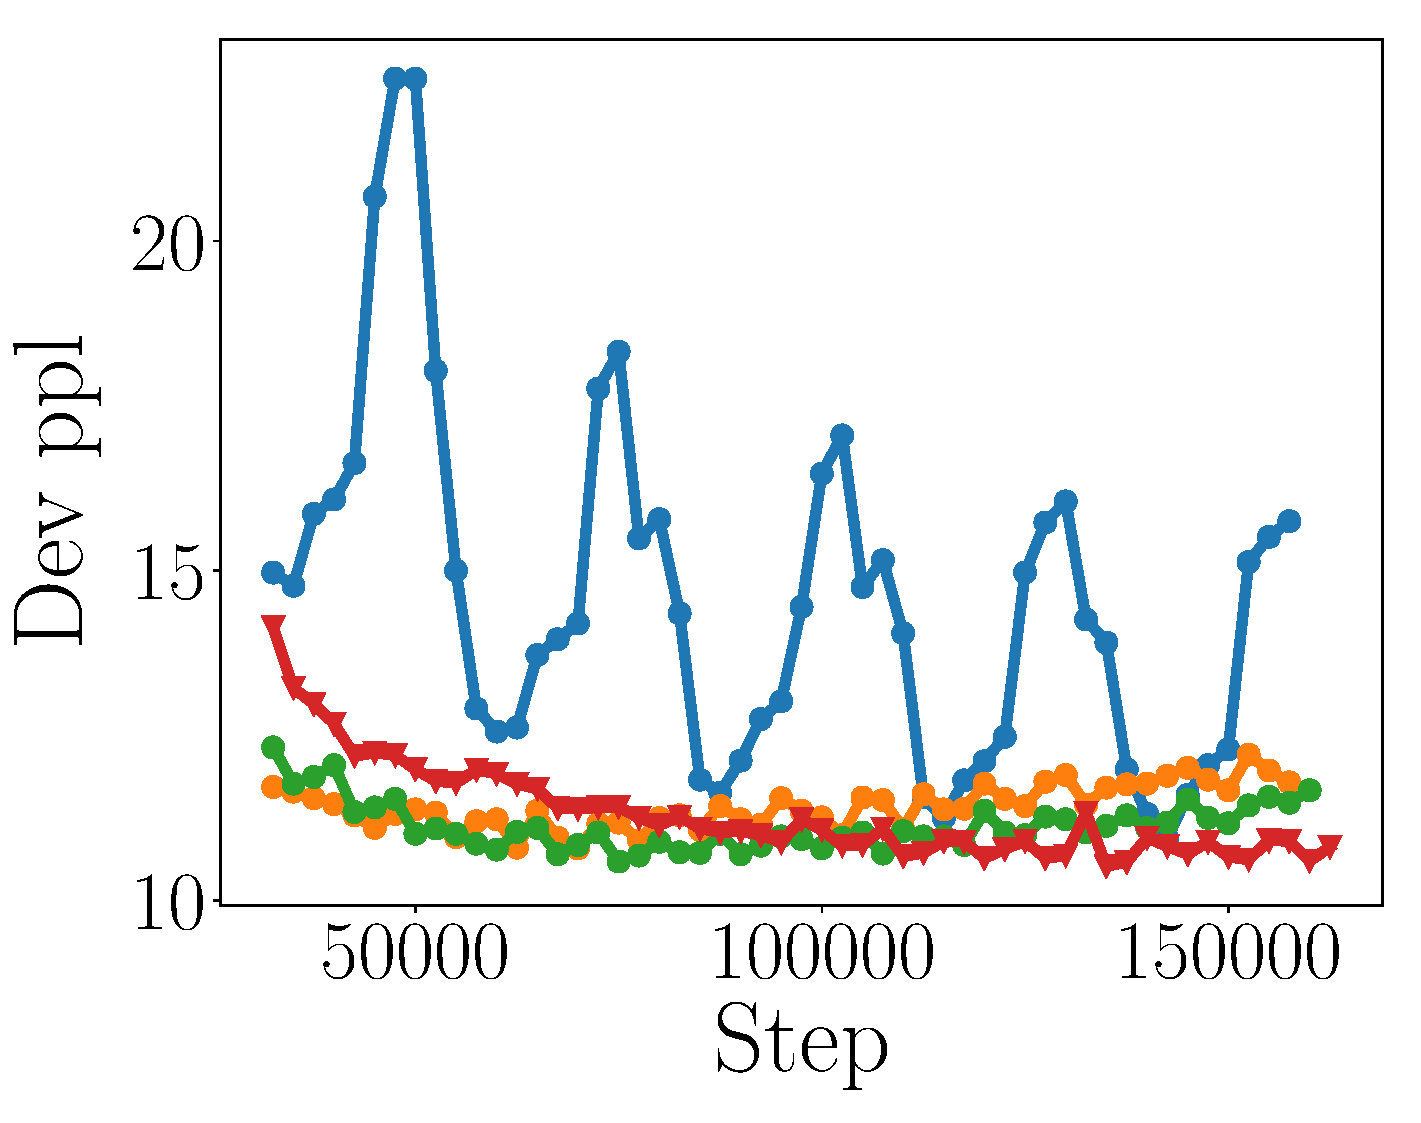
\includegraphics[width=0.245\columnwidth]{figs/aze_devppl_plot.eps}
  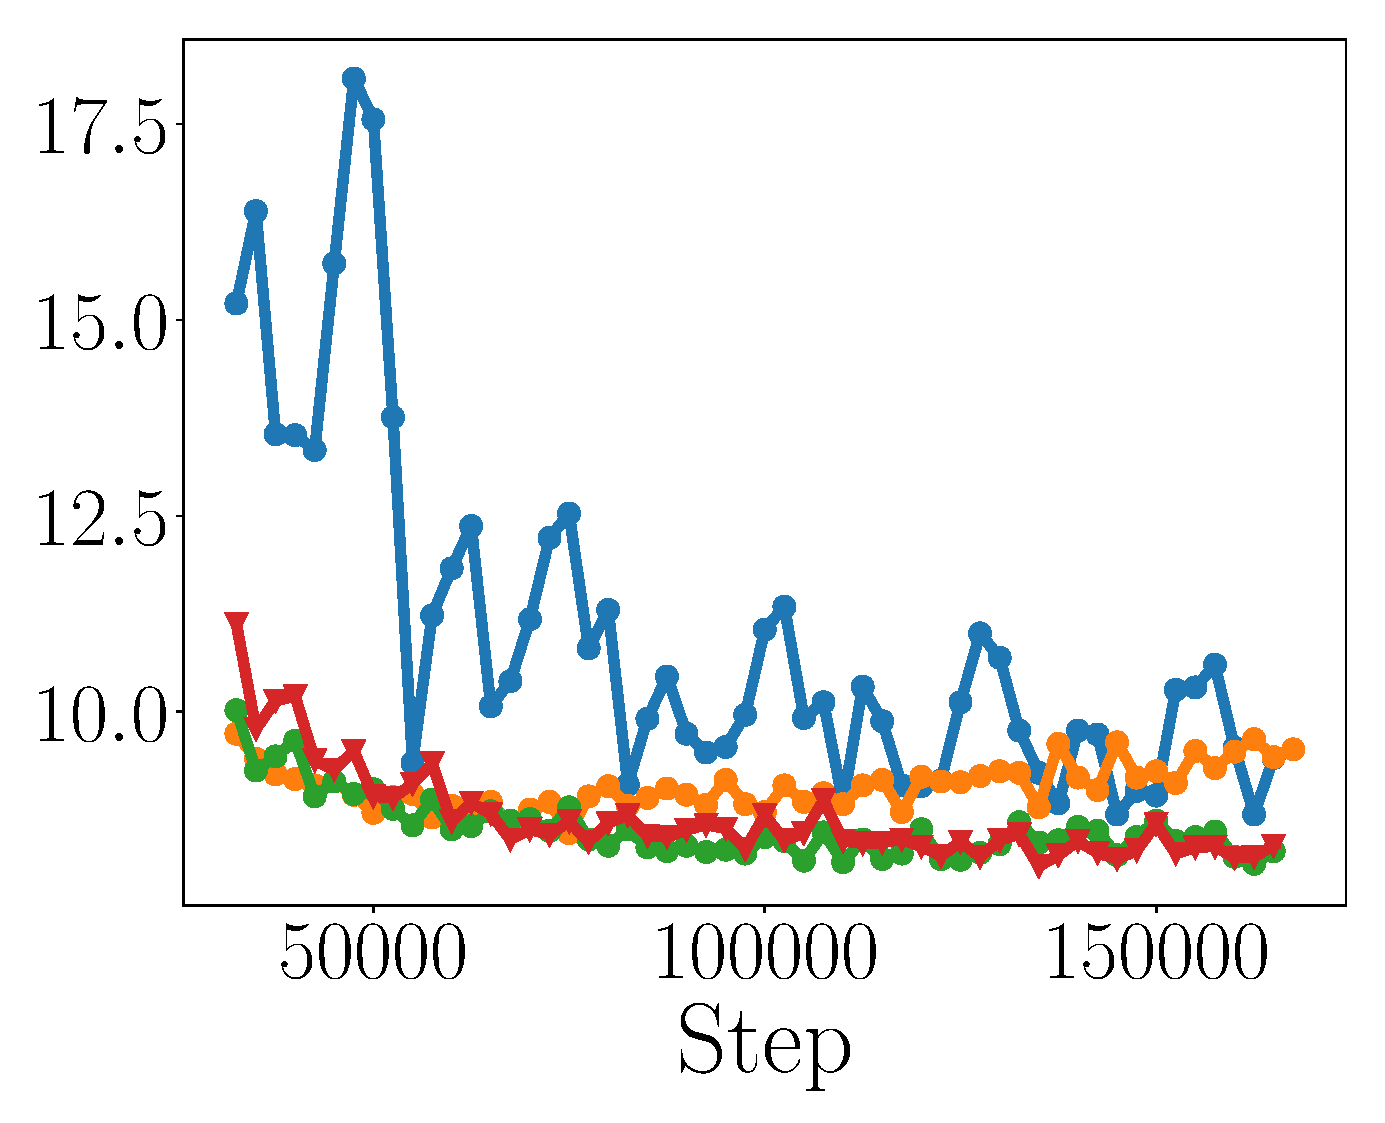
\includegraphics[width=0.23\columnwidth]{figs/bel_devppl_plot.eps}
  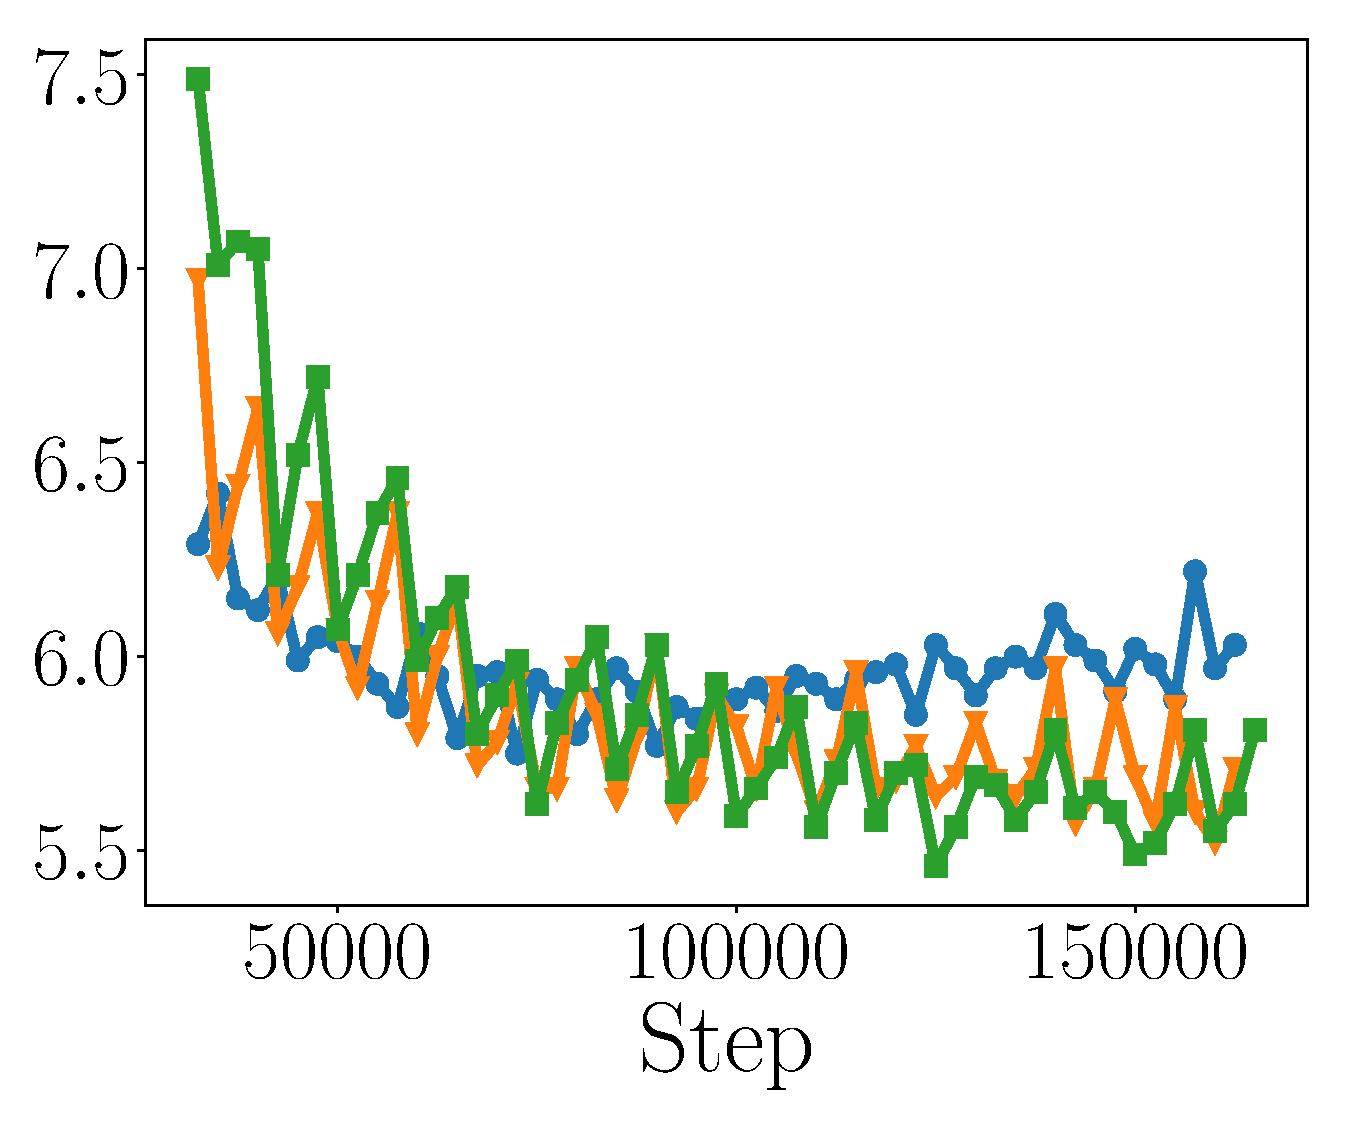
\includegraphics[width=0.23\columnwidth]{figs/glg_devppl_plot.eps}
  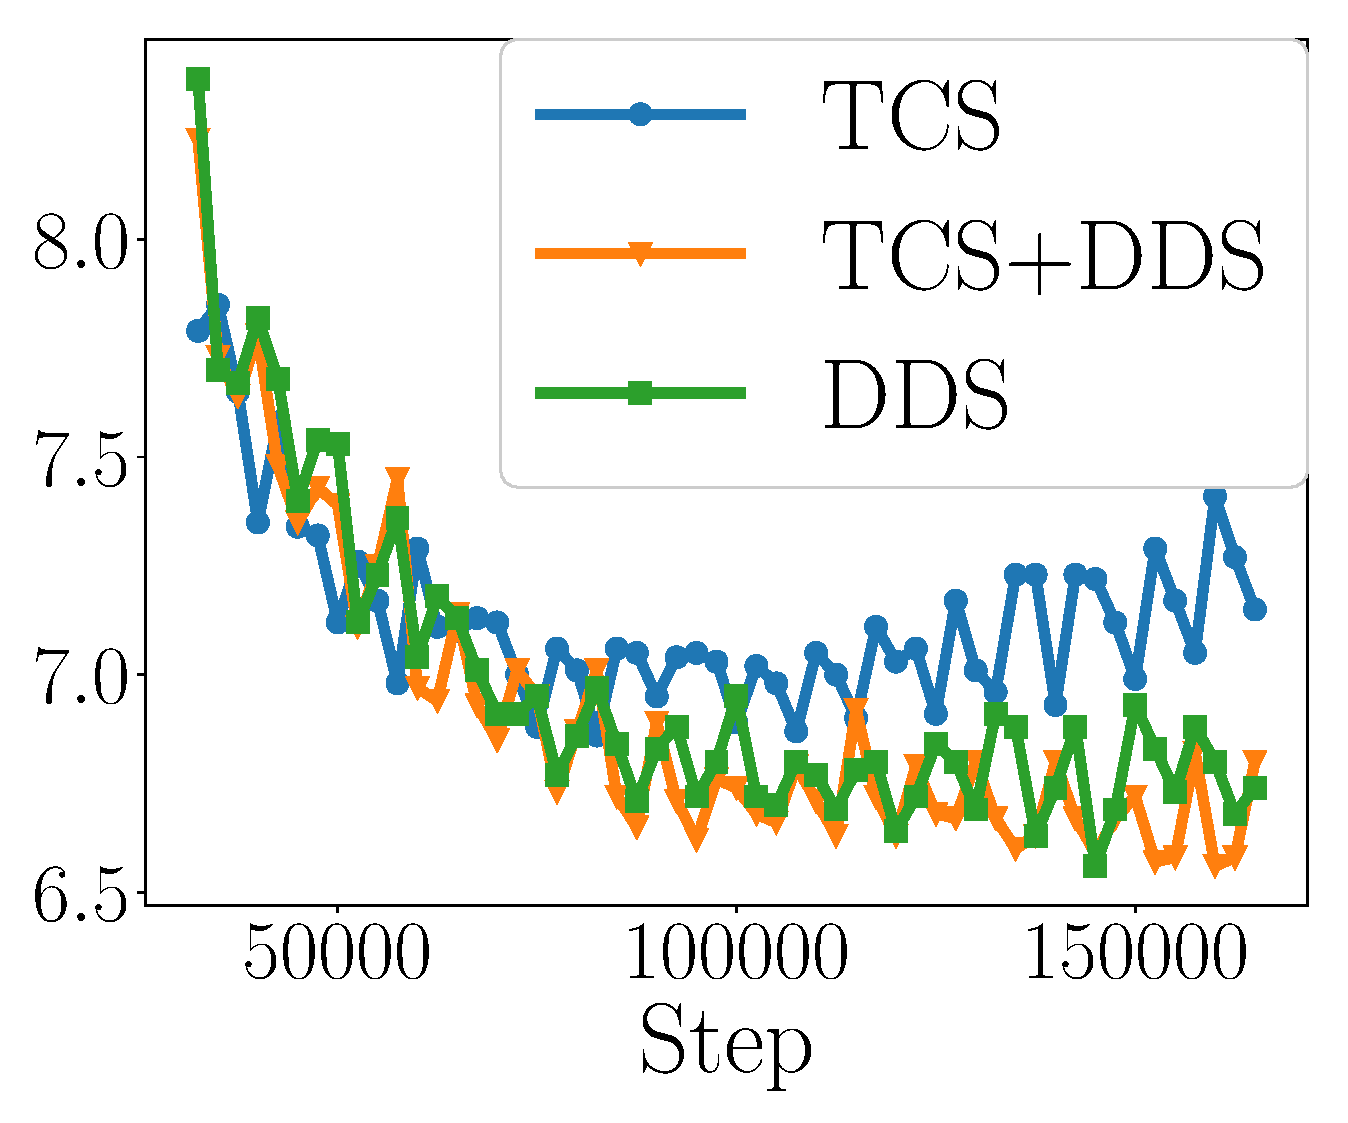
\includegraphics[width=0.23\columnwidth]{figs/slk_devppl_plot.eps}
  \captionof{figure}{\label{fig:nmt_converge}Development set perplexity vs. training steps. \textit{From left to right}: aze, bel, glg, slk.}
\end{center}
\paragraph{Training curve.} We plot the dev set perplexity over the course of training in Figure \ref{fig:nmt_converge}. DDS, with or without initialization with the heuristic distribution from TCS, allows the model to reach lower dev perplexity than TCS for all 4 languages.

\begin{center}
  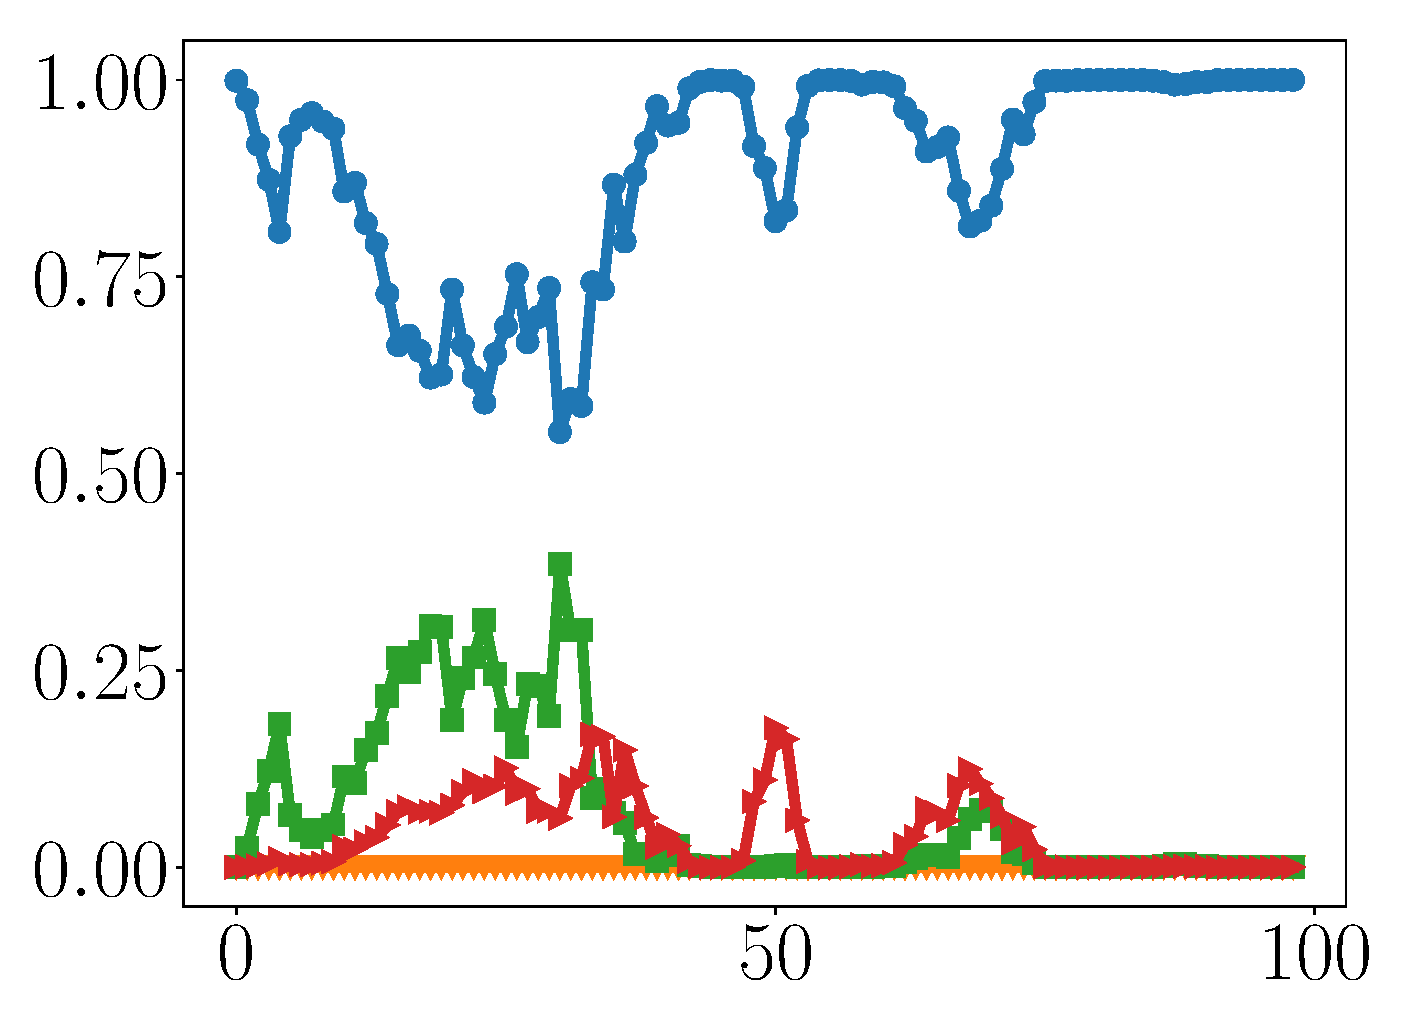
\includegraphics[width=0.22\columnwidth]{figs/aze_hs_probs_plot.eps}
  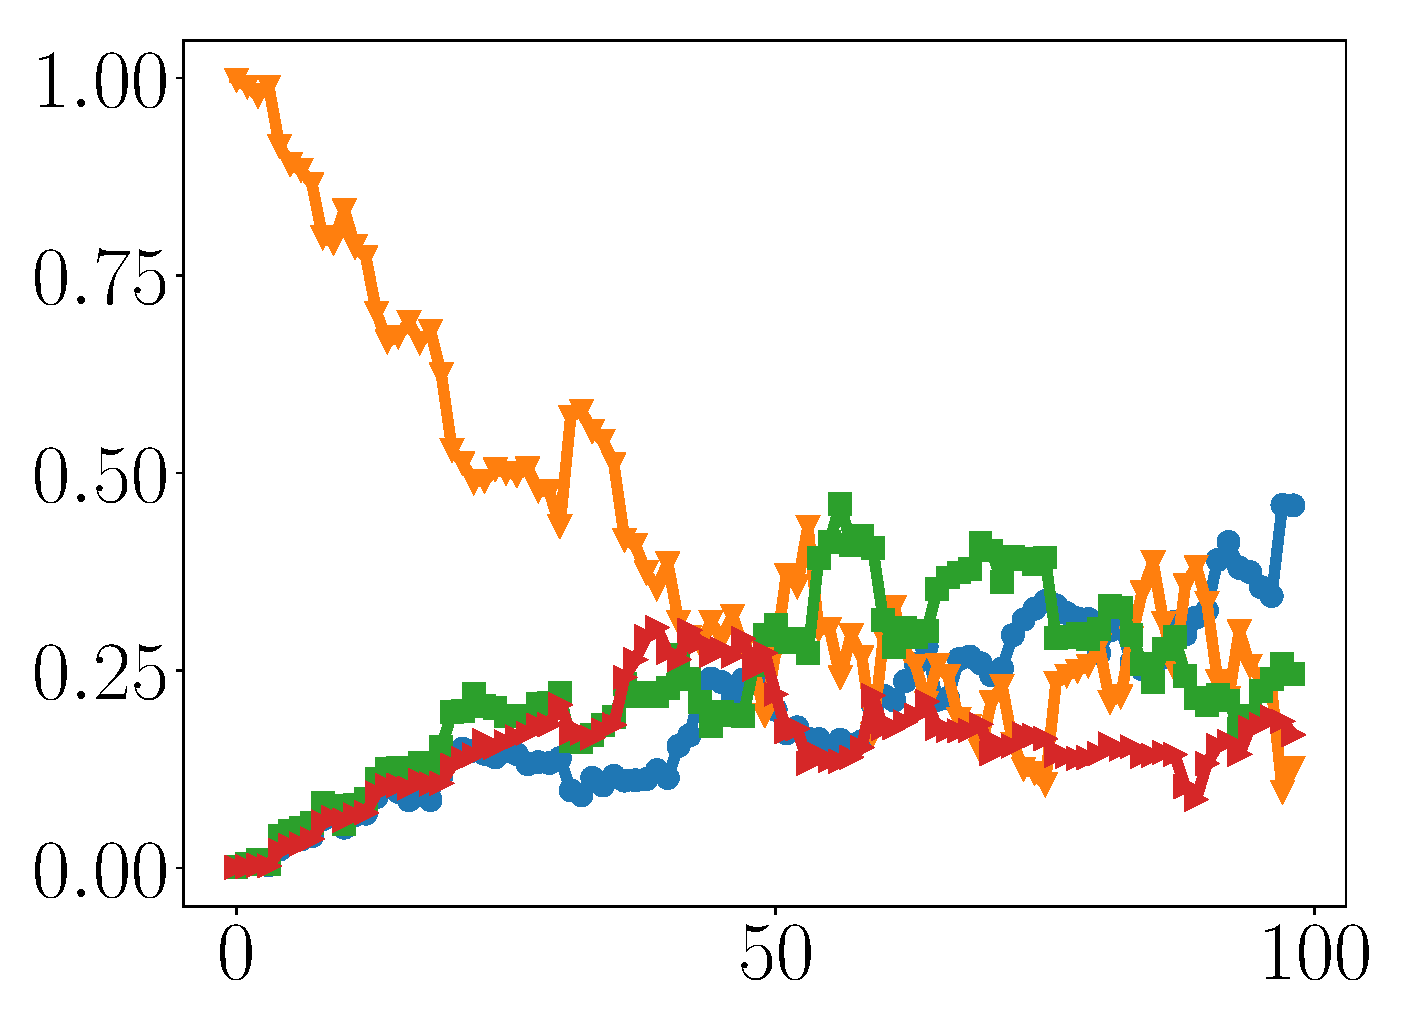
\includegraphics[width=0.22\columnwidth]{figs/bel_hs_probs_plot.eps}
  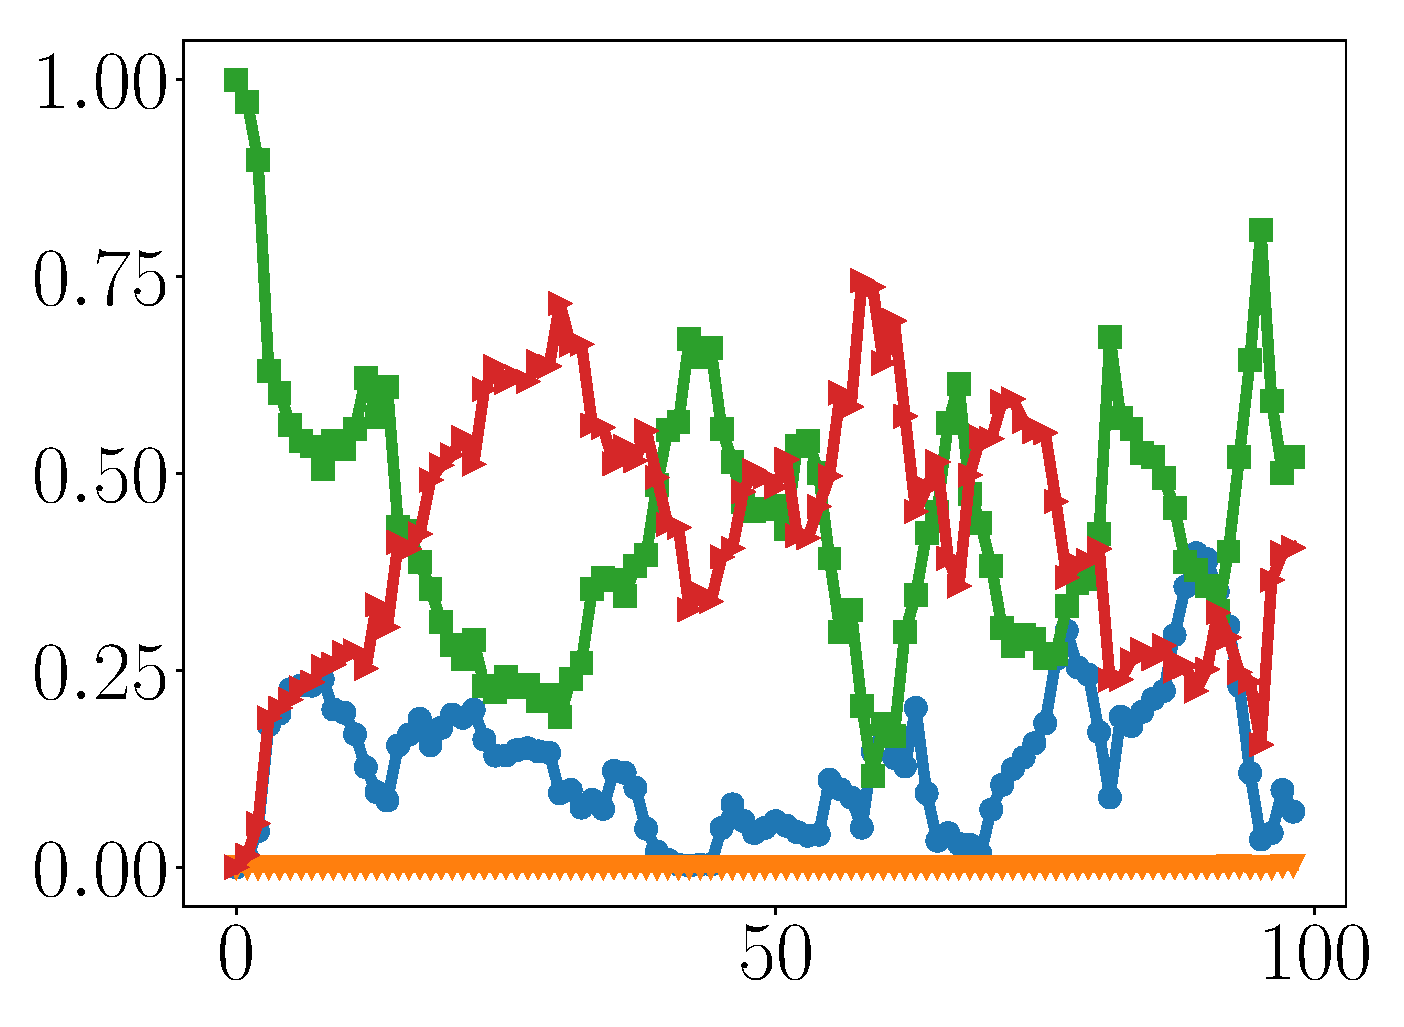
\includegraphics[width=0.22\columnwidth]{figs/glg_hs_probs_plot.eps}
  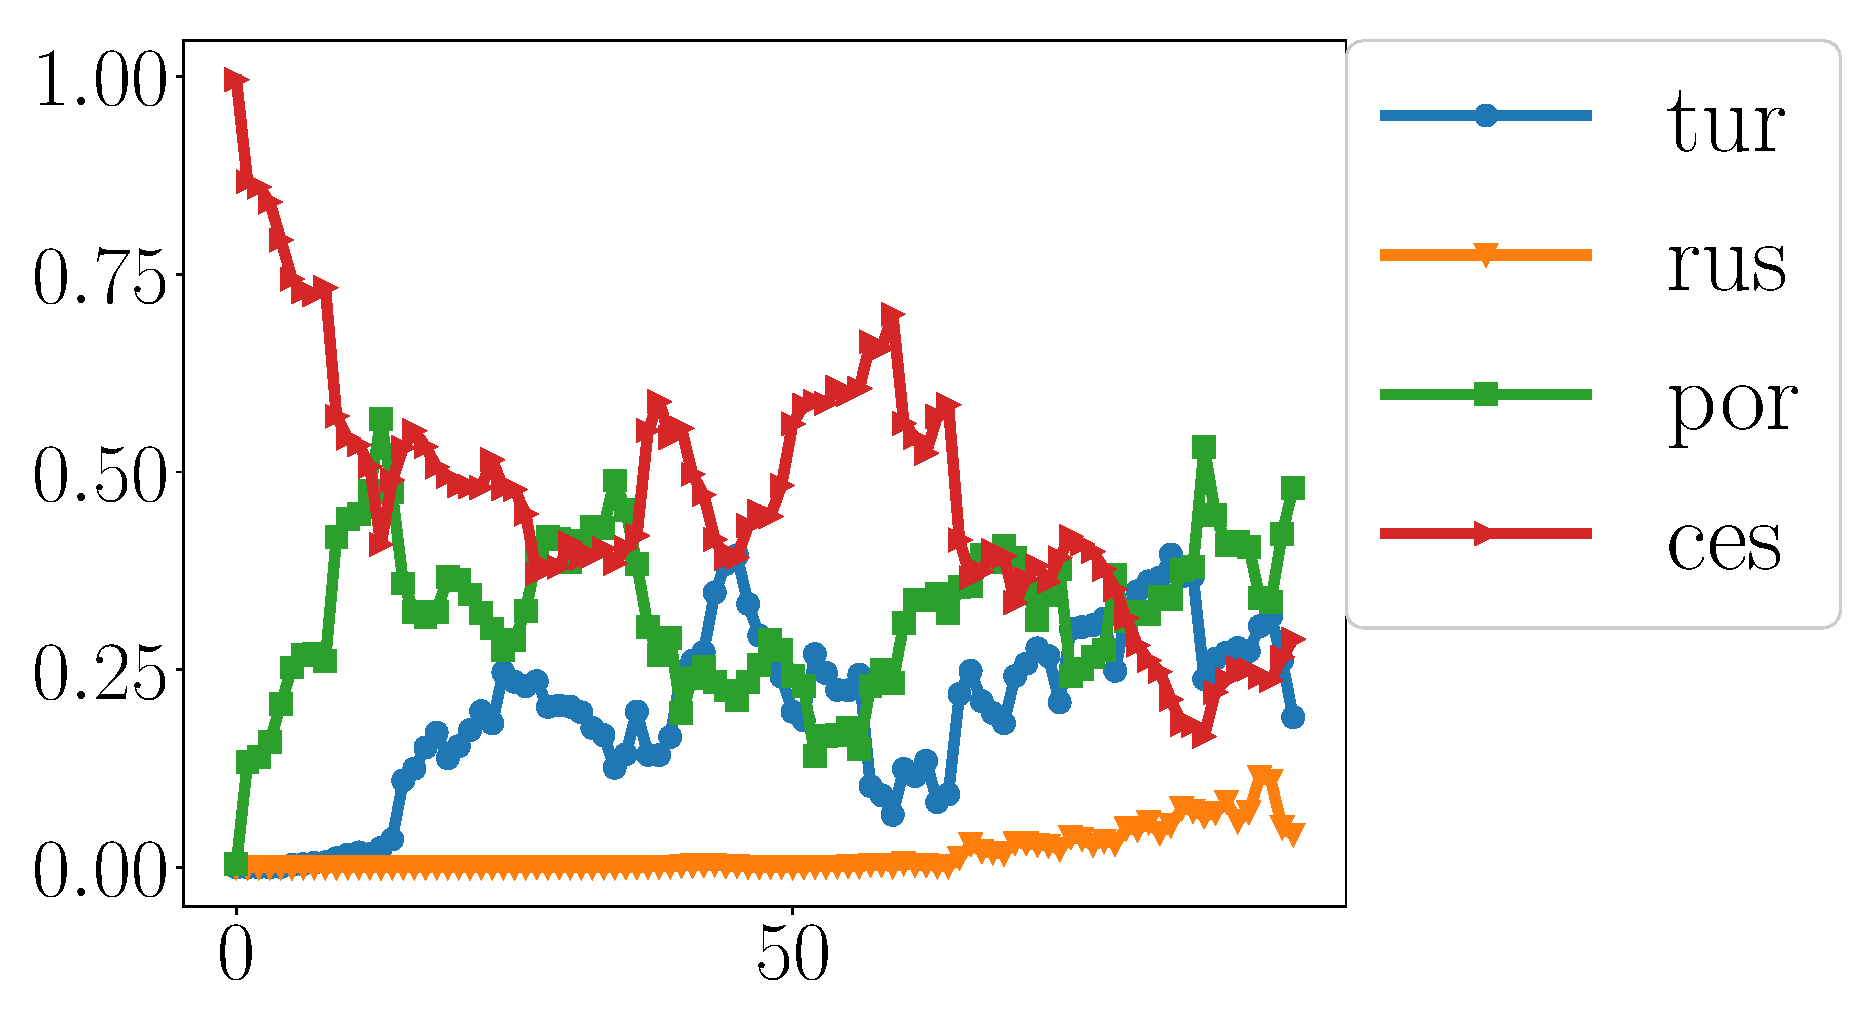
\includegraphics[width=0.29\columnwidth]{figs/slk_hs_probs_plot.eps}
  \captionof{figure}{\label{fig:nmt_distrib_hs}Language usage for TCS$+$DDS vs. training steps. \textit{From left to right}: aze, bel, glg, slk.}
\end{center}

\begin{center}
  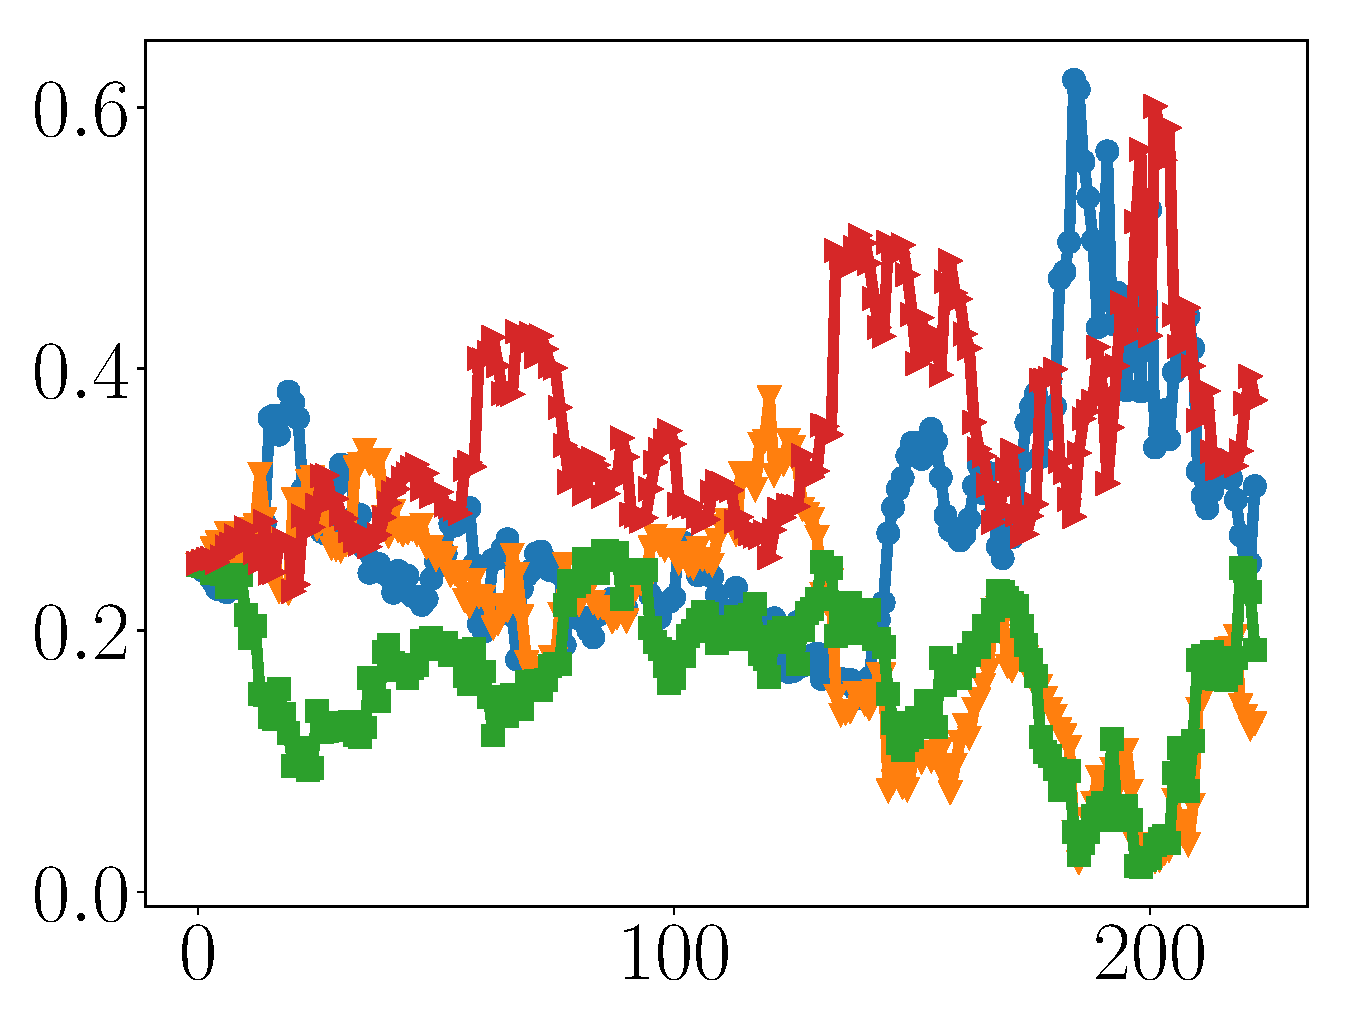
\includegraphics[width=0.22\columnwidth]{figs/aze_uni_probs_plot.eps}
  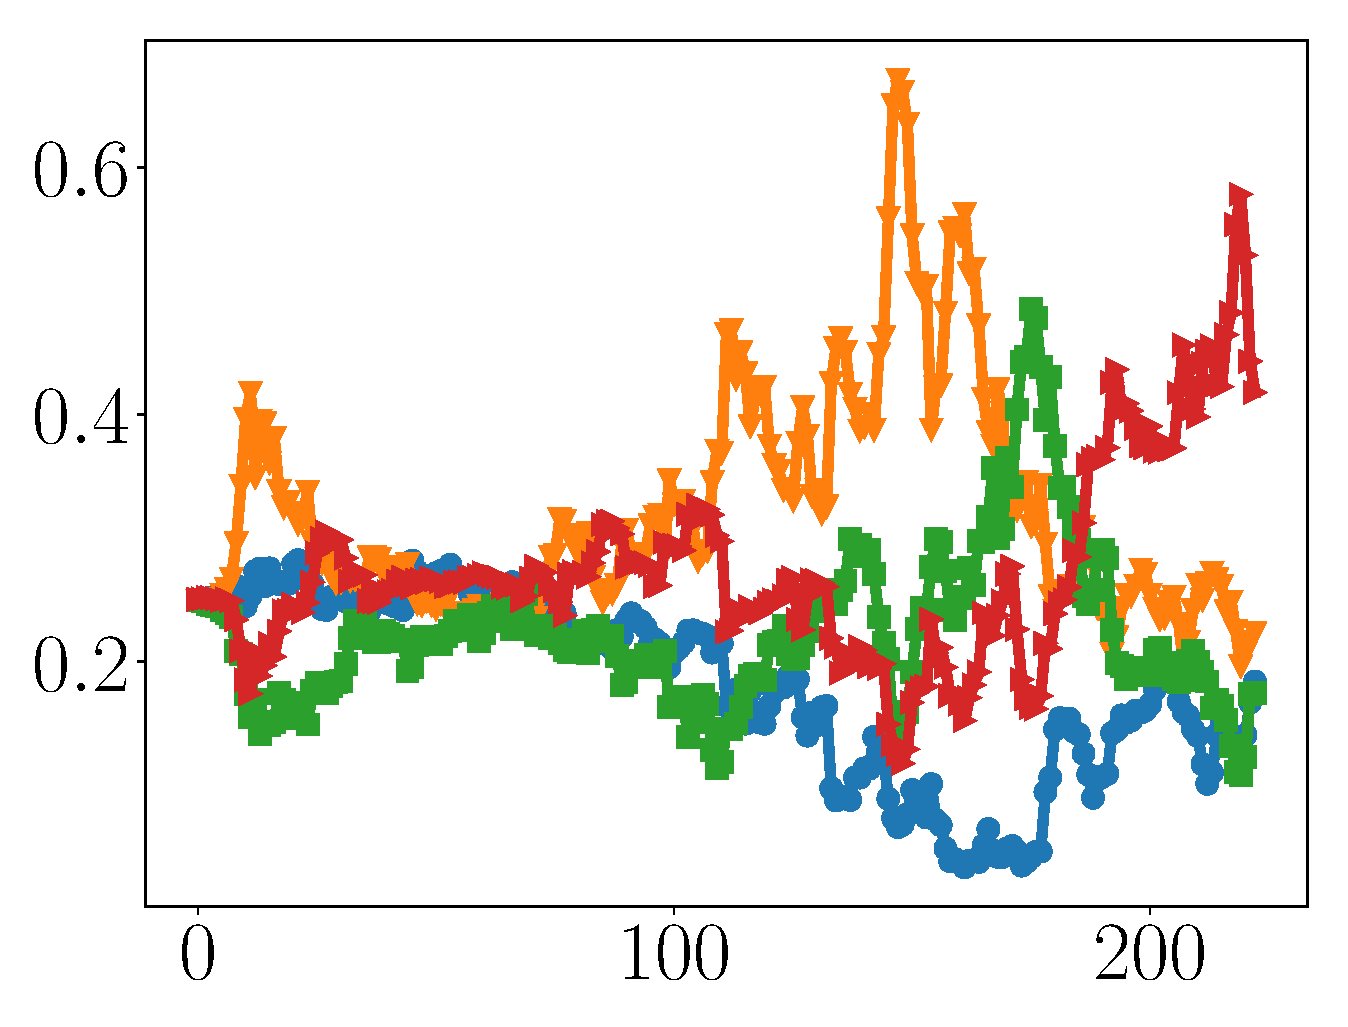
\includegraphics[width=0.22\columnwidth]{figs/bel_uni_probs_plot.eps}
  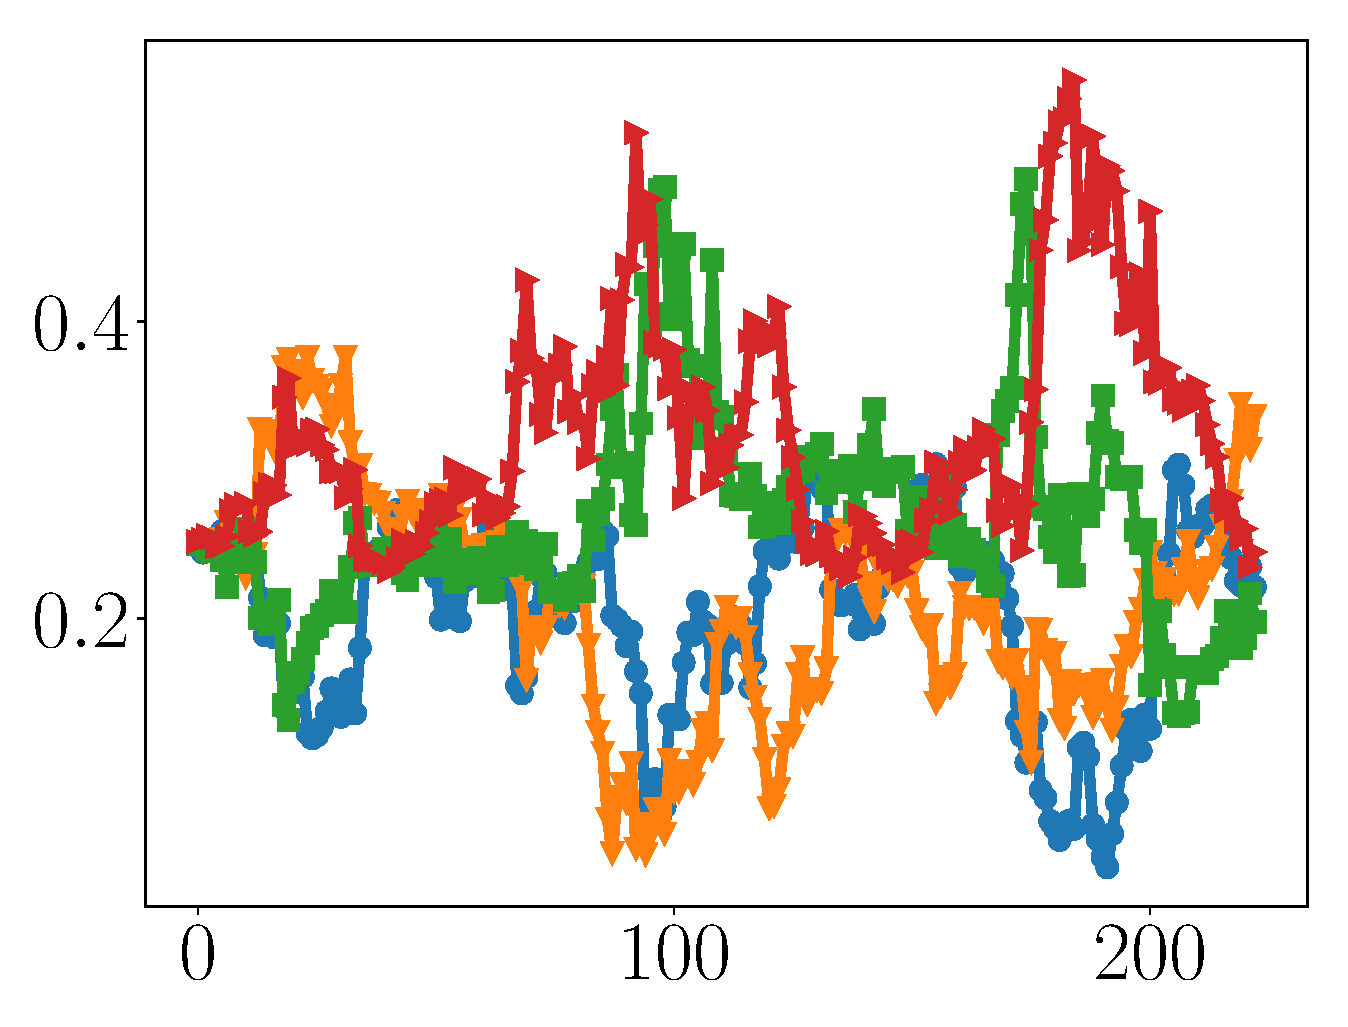
\includegraphics[width=0.22\columnwidth]{figs/glg_uni_probs_plot.eps}
  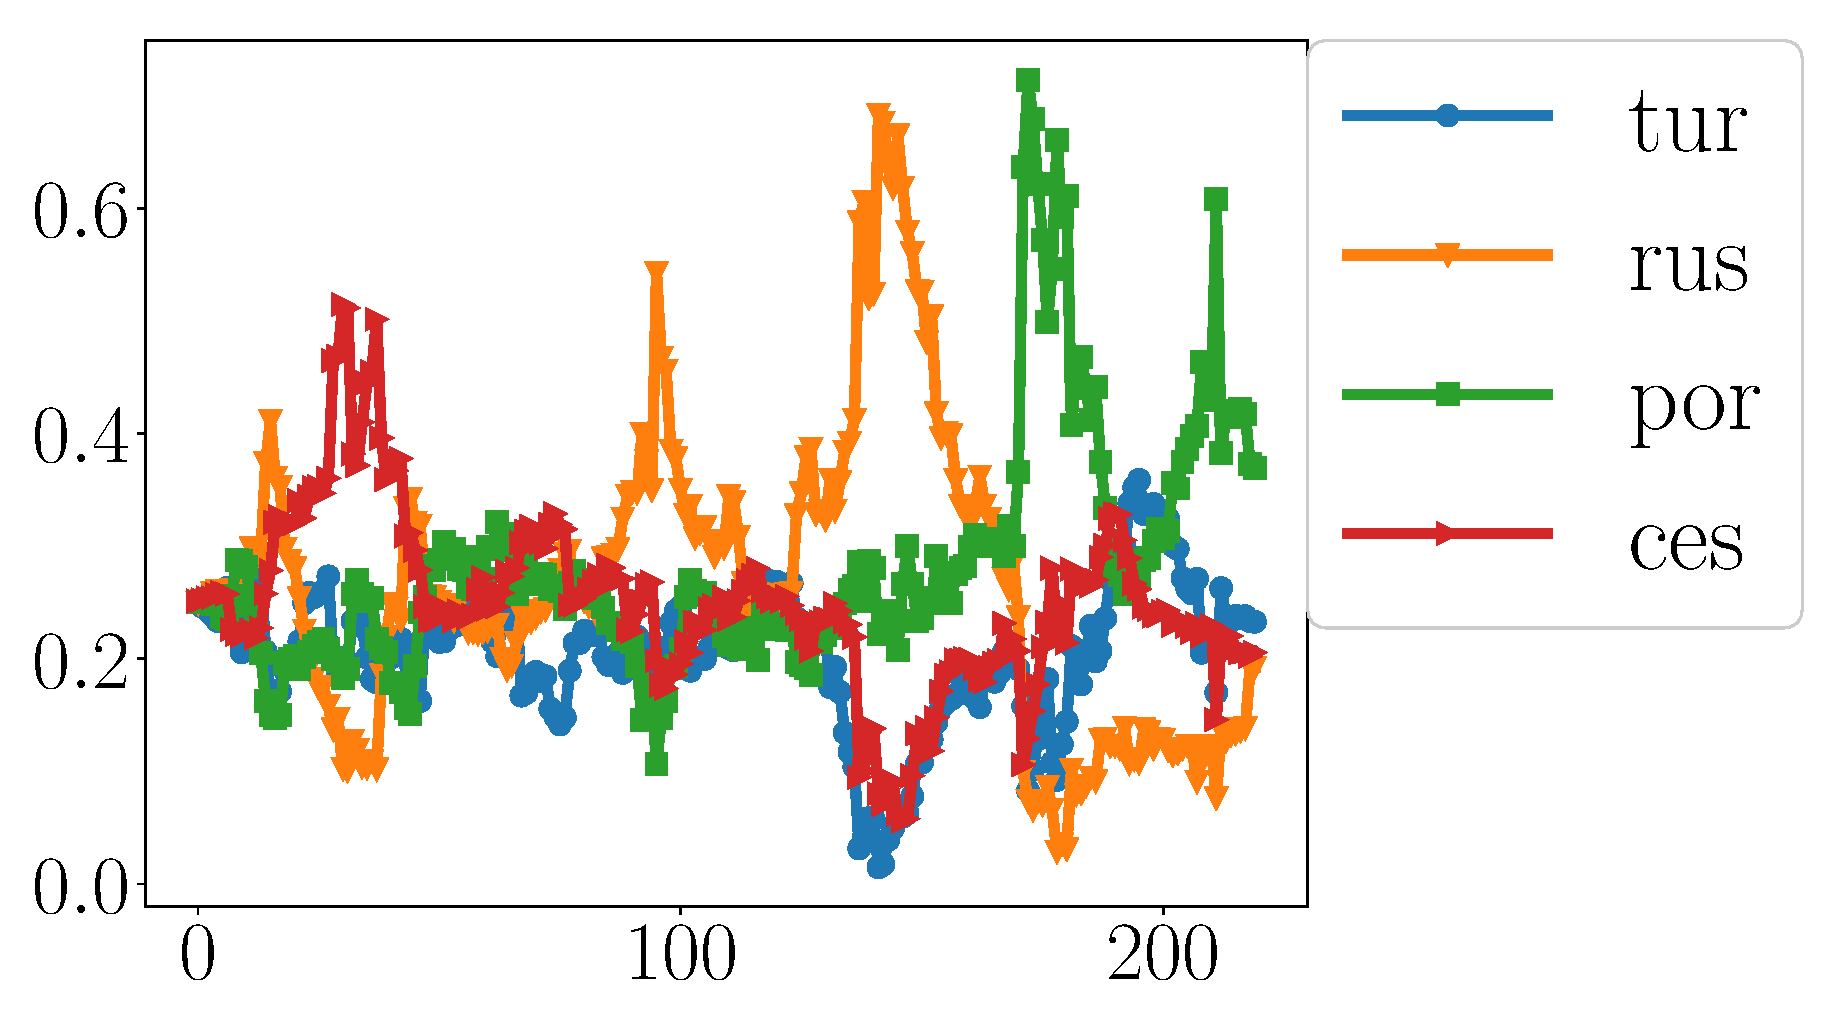
\includegraphics[width=0.29\columnwidth]{figs/slk_uni_probs_plot.eps}
  \captionof{figure}{\label{fig:nmt_distrib_uni}Language usage for Uniform$+$DDS vs. training steps. \textit{From left to right}: aze, bel, glg, slk.}
\end{center}
\paragraph{Learned Language Distribution} To analyze the learned language distribution, we plot the probability distribution of the four HRLs over the course of training. We focus on the four languages because they have the most amount of data and probably affect the model performance more.  Figure \ref{fig:nmt_distrib_hs} shows the change of language distribution for TCS+DDS. Since TCS selects the language with the most number of vocabulary overlap with the LRL, the distribution is initialized to focus on the most related HRL. For all four LRLs, the percentage of their most related HRL start to decrease as training begins. For aze, DDS quickly comes back to using the its most related HRL. However, for bel, DDS continues the trend of using all four languages. This shows that DDS is able to maximize the benefits of the multilingual data by having a more balanced usage of all languages. 
%For gig and slk, DDS learns to mainly use both por and ces, their corresponding HRL.

In Figure \ref{fig:nmt_distrib_uni}, we show a more interesting trend of DDS without heuristic initialization. For both aze and bel, our method learns to focus on their most related HRL after some training updates.
Interestingly, for bel, DDS learns to focus on both rus, the most related HRL for bel, and another language ces. Similarly for slk, DDS also learns to focus on ces, its most related HRL, and rus, although there is little vocabulary overlap between slk and rus. Since DDS does not rely on heuristics, such as vocabulary overlap between languages, it is able to discover better data usage strategies than the already strong heuristic methods such as TCS.
%Similar to the trend in Figure \ref{fig:nmt_distrib_hs}, glg tends to use both por, its most related HRL, and ces. 
